\documentclass[../main/main.tex]{subfiles}
\begin{document}

\chapter{Geometry in the spacetime}
Refer to \textsf{Carroll chap. 2} and \textsf{Nakahara chap. 5,7} for this chapter.\\

\section{Differential geometry of metric spaces}

\subsection{Manifolds}

\begin{definition}{}
$M$ is a $d$-dimensional differentiable manifold if
\begin{enumerate}
\item $M$ is a topological space
\item $M$ is provided with a family of pairs $\{(U_\alpha, \phi_\alpha)\}$
\item $\{U_\alpha\}$ is a family of open sets which covers $M$, that is,  $\bigcup_\alpha U_\alpha=M$. $\phi_\alpha$ is a homeomorphism from $U_\alpha$ onto an open subset $U_\alpha'$ of $\RR^d$;  
\begin{figure}[H]
\centering
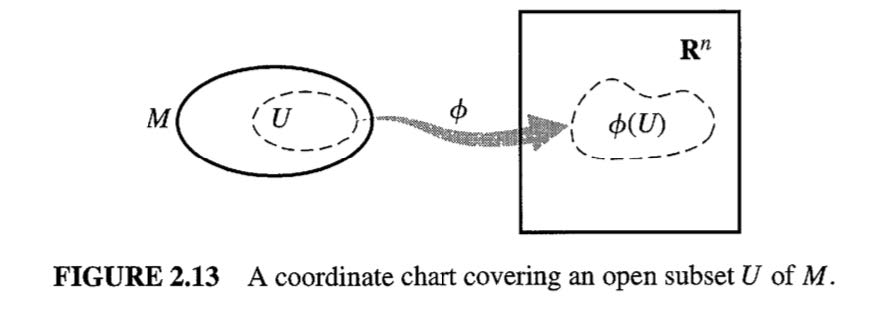
\includegraphics[width=7cm]{../img/chart-diff-geo.jpg}
\end{figure}
\item given $U_\alpha$ and $U_\beta$ such that $U_\alpha\cap U_\beta\neq\emptyset$, the map $\psi_{\alpha\beta}=\phi_\alpha\circ\phi_\beta^{-1}$ from $\phi_\beta(U_\alpha\cap U_\beta)$ to $\phi_\alpha(U_\alpha\cap U_\beta)$ is infinitely differentiable.
\begin{figure}[H]
\centering
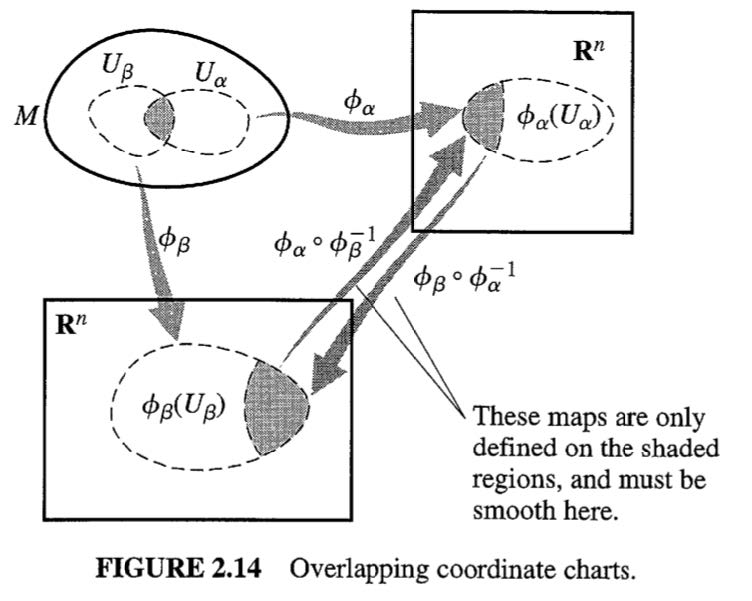
\includegraphics[width=7cm]{../img/compatible-chart-diff-geo.jpg}
\end{figure}
\end{enumerate}
The pair $(U_\alpha, \phi_\alpha)$ is called a \textbf{chart} while the whole family $\{(U_\alpha, \phi_\alpha)\}$ is called an \textbf{atlas}. The subset $U_\alpha$ is called the \textbf{coordinate neighbourhood} while $\phi_\alpha$ is the \textbf{coordinate function} or, simply, the \textbf{coordinate}. If $U_\alpha$ and $U_\beta$ overlap, two coordinate systems are assigned to a point in $U_\alpha\cap U_\beta$. Axiom (iv) asserts that the transition from one coordinate system to another be \emph{smooth} ($C^\infty$). The map $\psi_{\alpha\beta}=\phi_\alpha\circ\phi_\beta^{-1}$ is called \textbf{transition function}. The choice of an atlas is not unique, in particular for each manifold there are infinite equivalent choices of atlas. If the union of two atlases $\{(U_\alpha, \phi_\alpha)\}$ and $\{(V_\beta, \varphi_\beta)\}$ is again an atlas, these two atlases are said to be \textbf{compatible}. The compatibility is an equivalence relation, the equivalence class of which is called the \textbf{differentiable structure}.
\end{definition}

\begin{example}[$S^2$]
The two dimensional sphere $S^2$ given by the subset of $\RR^3$ defined by the equation
\[(X^1)^2+(X^2)^2+(X^3)^2=R^2\]
is a differentiable manifold. Notice that no single chart is possible, since the sphere is a closed set, thus cannot be found any homeomorphism with an open set of $\RR^2$, rather we need to define at least two charts. We can do this using \emph{stereographic coordinates}:
\begin{alignat*}{4}
\phi_N\,:\,U_N=&&S^2\setminus\{(0,0,-R)\}&&\quad\longrightarrow\quad &\phi_N(U_N)\simeq\RR^2\\
&&(X^1,X^2,X^3)&&\quad\longmapsto\quad&\p{x_N^1=\frac{2X^1}{R+X^3},\,x_N^2=\frac{2X^2}{R+X^3}}
\end{alignat*}
\begin{figure}[H]
\centering
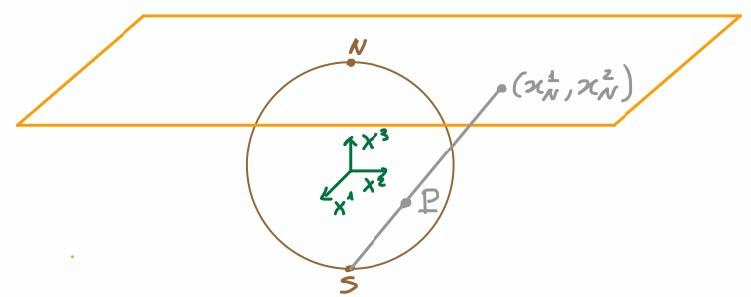
\includegraphics[width=7cm]{../img/stereo-coord-2sphere.jpg}
\end{figure}
\noindent where the chart is defined for all points of $S^2$ beside the south pole. Analogously, removing the north pole:
\begin{alignat*}{4}
\phi_S\,:\,U_S=&&S^2\setminus\{(0,0,R)\}&&\quad\longrightarrow\quad &\phi_S(U_S)\simeq\RR^2\\
&&(X^1,X^2,X^3)&&\quad\longmapsto\quad&\p{x_S^1=\frac{2X^1}{R-X^3},\,x_S^2=\frac{2X^2}{R-X^3}}
\end{alignat*}
We can see that transition functions are smooth:
\begin{align*}
\phi_S\circ\phi_N^{-1}\,:\,(x_N^1,x_N^2)\quad\longmapsto\quad	 \begin{cases}
x_S^1=\frac{4x_N^1}{(x_N^1)^2+(x_N^2)^2}\\
x_S^2=\frac{4x_N^1}{(x_N^2)^2+(x_N^2)^2}
\end{cases}
\end{align*}
\end{example}

\begin{example}[$S^n$]
The two dimensional sphere $S^n$ given by the subset of $\RR^{n+1}$ defined by the equation
\[(X^1)^2+(X^2)^2+\dots+(X^{n+1})^2=R^2\]
is a differentiable manifold. Notice that again no single chart is possible, rather we need to define several charts. This time, instead of stereographic coordinates (which works too) we use \emph{angular coordinates}:
\begin{align*}
\begin{cases}
X^{n+1}&=R\cos\theta_1\\
X^n&=R\sin\theta_1\cos\theta_2\\
X^{n-1}&=R\sin\theta_1\sin\theta_2\cos\theta_3\\
&\vdots\\
X^2&=R\sin\theta_1\dots\cos\theta_n\\
X^1&=R\sin\theta_1\dots\sin\theta_n
\end{cases}
\qquad\text{with}\quad0<\theta_1,\dots,\theta_{n-1}<\pi\,,\quad0<\theta_n<2\pi
\end{align*}
\begin{figure}[H]
\centering
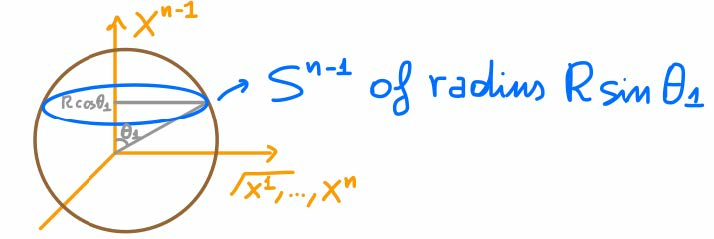
\includegraphics[width=8cm]{../img/chart-N-sphere-angular.jpg}
\end{figure}
\noindent Notice that this coordinates degenerate at $\theta_1,\dots,\theta_{n-1}=0,\pi$, therefore this chart do not cover the entire $S^n$. For example coordinates for the submanifold $S^{n-2}=S^n\cap\{X^1=X^2=0\}$ (i.e. $\theta_{n-1}=0$) are not well defined. In order to cover the full sphere we can use charts with ``rotated'' angular coordinates that covers subsets of $S^n$ where the previous chart is not well defined. 

\end{example}


\begin{example}[$n$-dim. de Sitter spacetime]
The so called \textbf{$n$-dim. de Sitter spacetime}, indicated by dS$n$, is the manifold defined as the subset of  $R^{n+1}$ with equation:
\[|\vec X|^2-T^2=L^2\]
where $\vec X=(X^1,\dots,X^n)$ are $n$ space coordinates while $T$ is a time coordinate. 
\begin{figure}[H]
\centering
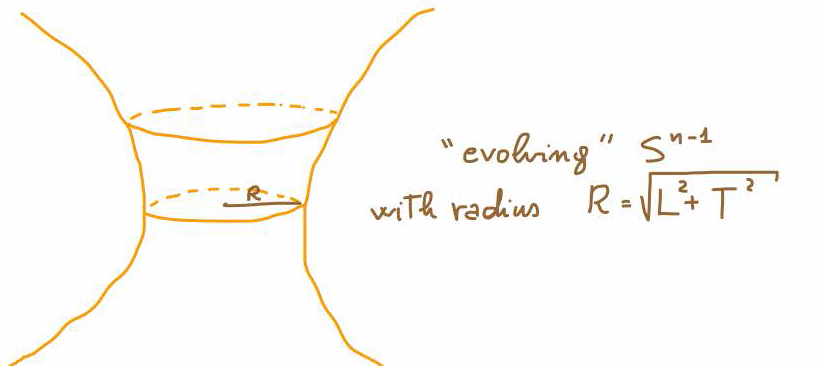
\includegraphics[width=8cm]{../img/de-Sitter-manifold.jpg}
\end{figure}
\noindent It's clear that this manifold takes the form of an hyperboloid. 
We may also introduce local coordinates on the manifold $x^\mu=(x^0,x^i)=(t,x^i)$. First we introduce coordinates $t$ and $\hat X^I$ such that
\begin{align*}
T&=L\sinh t\\
X^I&=L\cosh \hat X^I
\end{align*}
with $\sum_{I=1}^n(\hat X^I)^2=1$, i.e. coordinates $\{\hat X^I\}$ define a sphere $\hat S^{n-1}$ with radius $\hat R=1$. Then, $\hat S^{n-1}$ can be covered using some atlas (e.g. using stereographic or angular coordinates), defining local coordinates $\{x^i\}$ on $\hat S^{n-1}$. In this way, taking into account also $x^0=t$, we introduce coordinates $x^\mu$ over dS$n$. \\
What we have done is just slice dS$n$ into spheres (circumferences in the figure) and then parametrize them as we already know by previous examples. 

\end{example}

Up to this point, we want to stress the fact that for these manifolds only pathches, topological and differential structure have been specified. No notion of distance has been introduced yet. 


\subsection{Calculus on Manifolds}


\begin{definition}{}
A \textbf{scalar field} is defined as a function
\begin{alignat*}{4}
F\,:\,&&M&&\quad\longrightarrow\quad&\RR\qquad(\text{or }\CC)\\
&&p&&\quad\longmapsto\quad&F(p)
\end{alignat*}
Let $(U,\phi)$ be a patch for $M$ with local coordinates $x^\mu$, then for each $p\in U$ we can define the \emph{local form} of F
\begin{alignat*}{4}
f=F\circ\phi^{-1}\,:\,&&\RR^d&&\quad\longrightarrow\quad&\RR\qquad(\text{or }\CC)\\
&&x&&\quad\longmapsto\quad&F(\phi^{-1}(x))
\end{alignat*}
If we consider a different patch $(\tilde U,\tilde \phi)$ associated to local coordinates $\tilde x^\mu$, and the local form of $f$ in this patch $\tilde f=F\circ\tilde\phi^{-1}$, then its immediate that following \textbf{transformation rule for a scalar field} holds:
\[\boxed{\tilde f(\tilde x)=f(x)}\]
where $\tilde x$ are the coordinates for $M$ using the patch $(\tilde U,\tilde \phi)$.
\end{definition}

Pragmatically, we will not distiguish between $F$ and its local form $f(x)$ and use the latter.
%
\begin{definition}{}
We define a \textbf{vector field}
\begin{alignat*}{4}
V\,:\,&&M&&\quad\longrightarrow\quad&TM\\
&&p&&\quad\longmapsto\quad& V^\mu(p)\partial_\mu\big\vert_p
\end{alignat*}
where $V^\mu$ is a set of  functions called \textbf{components of the vector field} and $\partial_\mu\equiv\frac\partial{\partial x^\mu}\vert_p$ are partial derivatives defined respect to the local coordinates in $p$ given by some patch, and they can be applied to any scalar field. The set $TM$ is a set of derivative operators that will be defined later. If functions $V^\mu$ are differentiable then the vector field is said \textbf{smooth}, and this condition is independent from the choice of the patch. The element $V(p)$ for some point $p\in M$ is said to be a  \textbf{vector in $p$} and the set of all vectors attached to a point $p$ (for all possible vector fields) is called \textbf{tangent space in $p$}, denoted by $T_pM$. Each $V^\mu(p)\partial_\mu\vert_p$ can be interpreted as a vector in $p$ with components $(V^1(p),V^2(p),\dots,V^n(p))$.

Suppose that $x^\mu$ and $\tilde x^\mu$ are local coordinates on two subsets $U$ and $\tilde U$. 
Notice that since transition functions for different charts are smooth, then in $U\cap\tilde U$ the Jacobian of the transition function $\frac{\partial\tilde x^\mu}{\partial x^\nu}(p)$ must be invertible, with inverse $\frac{\partial x^\mu}{\partial\tilde x^\nu}(p)$. The transformation rule for partial derivatives is then given by the differentiable application $\partial_\mu=\frac{\partial\tilde x^\nu}{\partial x^\mu}\tilde\partial_\nu$ and similarly the \textbf{transformation rule for a vector field} is 
\[\hspace{1cm}
\begin{split}
 &V^\mu\partial_\mu=V^\mu\frac{\partial\tilde x^\nu}{\partial x^\mu}\tilde\partial_\nu=\tilde V^\nu\tilde\partial_\mu\\
&\boxed{\tilde V^\mu(\tilde x)=\frac{\partial\tilde x^\mu}{\partial x^\nu}V^\nu(x)}
\end{split}
\hspace{1cm}
\raisebox{-2cm}{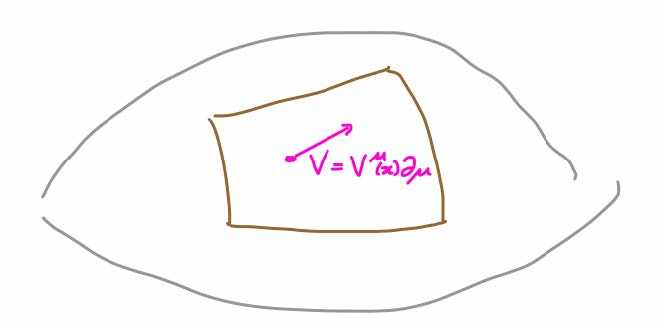
\includegraphics[width=5.5cm]{../img/tangent-vector.jpg}}
\]
Notice that this application reduce to the Minkowski rule for Poincaré transformations $\tilde x^\mu={\Lambda^\mu}_\nu x^\nu+\alpha^\mu$. 
Here is a pictorial representation of a smooth vector field on a sphere:
\begin{figure}[H]
\centering
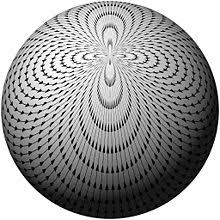
\includegraphics[width=5cm]{../img/example-vector-field.jpg}
\end{figure}

Starting from a manifold $M$ and a vector field $V$, we can define \textbf{integral curves}
\begin{alignat*}{4}
\gamma\,:\,&&\RR\supset I&&\quad\longrightarrow\quad&\gamma(I)\subset M\\
&&\lambda&&\quad\longmapsto\quad &\gamma(\lambda)
\end{alignat*}
such that
\[\frac{\de \gamma^\mu}{\de\lambda}(\lambda)=V^\mu(\gamma(\lambda))\]
\begin{figure}[H]
\centering
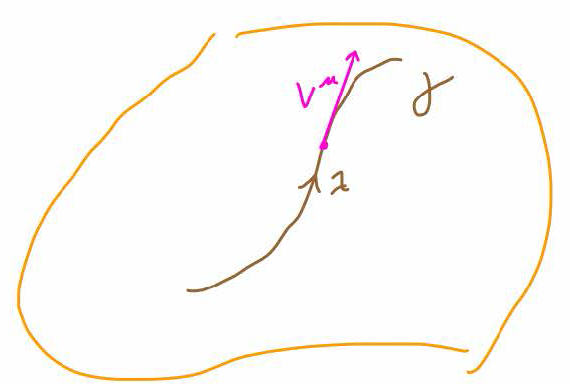
\includegraphics[width=4cm]{../img/integral-curve.jpg}
\end{figure}
\noindent Notice that the latter equation describes a set of first order differential equations with unique solution for a given initial conditions. The set of all integral curves, for different initial coordinates, is called the \textbf{flow} of the vector field.
\begin{figure}[H]
\centering
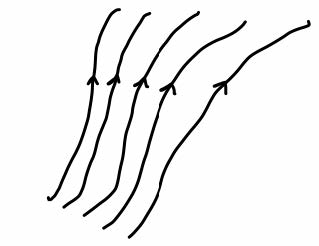
\includegraphics[width=2.5cm]{../img/flow-vector-field.jpg}
\end{figure}
\noindent We can then regard $V(p)$ as defining a directional derivative in $p$ of any smooth scalar field $f$ along the integral curve of $V$ that goes through $p=\gamma(\lambda_p)$ :
\[V(f)(p)\equiv V^\mu(p)\partial_\mu f(p)=\frac{\de \gamma^\mu}{\de\lambda}(p)\partial_\mu f(p)=\frac{\de (f\circ\gamma)}{\de\lambda}(\lambda_p)\]
and this can be interpreted as the derivative of the restriction of $f$ along $\gamma$. This also allows a better interpretation of tangent vectors as derivative operators that can be applied to scalar fields. 

At each point $p\in M$ the tangent space $T_pM$ is a $d$-dimensional vector space and $\partial_\mu\big\vert_p\equiv\frac\partial{\partial x^\mu}\big\vert_p$ provide the coordinate basis associated with the local coordinates $x^\mu$, called \textbf{coordinate basis}. However we could take any other basis of linearly independent vectors $e_a=e_a^\mu(x)\partial_\mu\in T_pM$, $a=1,\dots,d$ so that $V(x)=V^a(x)e_a=V^\mu(x)\partial_\mu$ with $V^\mu(x)=e_a^\mu(x)V^a(x)$. Often indices $a$ are called \emph{``local''} (or \emph{``flat''} in GR) \emph{indices}, while $\mu$ are called \emph{``curved'' indices}.

The collection of the tangent spaces in each point $p\in M$ is called \textbf{tangent bundle} $TM$
\[TM=\bigcup_{p\in M}T_pM
\hspace{1.5cm}
\raisebox{-1cm}{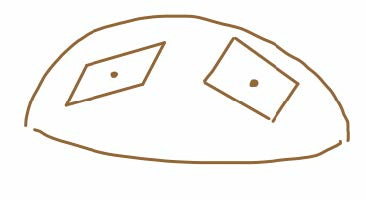
\includegraphics[width=3cm]{../img/vector-bundle.jpg}}
\]
\noindent Notice that this is a $2d$-dimensional manifold. A vector field $V$ can be also define as a function between the manifold and a bundle, i.e. a \textbf{section}. In particular a vector field is a section of the vector bundle
\begin{alignat*}{4}
V\,:\,&&M&&\quad\longrightarrow\quad&TM\\
&&p&&\quad\longmapsto\quad &X_p\in T_pM
\end{alignat*}
\end{definition}

\begin{example}
Let's consider the vector field $V=\sin\theta\partial_\phi$ where we used spherical coordinates $(x^1,x^2)=(\theta,\phi)$. Its components are
\vspace{-0.5cm}
\[V^\mu=(V^1,V^2)\equiv(V^\theta, V^\phi)=(0,\sin\theta)
\hspace{0.5cm}
\raisebox{-2cm}{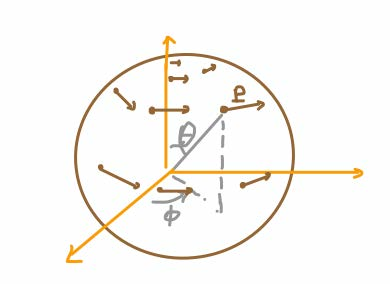
\includegraphics[width=4cm]{../img/vector-field-sintheta.jpg}}
\]
\end{example}













\end{document}